\documentclass[11pt,a4paper]{article}

\usepackage[T1]{fontenc}
\usepackage[utf8]{inputenc}
\usepackage{lmodern}
\usepackage{microtype}
\usepackage[margin=2.5cm]{geometry}
\usepackage{amsmath,amssymb,amsthm,mathtools,bm}
\usepackage{booktabs}
\usepackage{graphicx}
\usepackage[numbers,sort&compress]{natbib}
\usepackage{xcolor}
\usepackage[hidelinks]{hyperref}
\hypersetup{
  pdftitle={A sharp weak-driving phase-lag bound for a symmetric three-state Markov cycle},
  pdfauthor={Xiaojian Zeng},
  pdfsubject={Linear response of a periodically driven three-state Markov process},
  pdfkeywords={stochastic thermodynamics, Markov process, linear response, phase lag, spectral gap}
}

\newcommand{\Aobs}{\mathcal{A}}
\newcommand{\Bobs}{\mathcal{B}}
\newcommand{\eps}{\varepsilon}
\newcommand{\RR}{\mathbb{R}}
\DeclareMathOperator{\Var}{Var}
\newtheorem{result}{Result}

\title{A sharp weak-driving phase-lag bound for a symmetric three-state Markov cycle}
\author{Xiaojian Zeng\\
\small PBC School of Finance, Tsinghua University, Beijing 100190, China\\
\small \texttt{xiaojianzeng@foxmail.com}}
\date{}

\begin{document}
\maketitle

\begin{abstract}
Periodically driven stochastic systems lag behind their driving protocol. A generalized
phase lag has a sharp kinetic bound for two-state systems, while its extension to
multistate networks is open. We treat the smallest complete cycle with a common kinetic
prefactor and symmetric local-detailed-balance splitting. For arbitrary finite static
offsets and arbitrary non-gauge finite Fourier driving, the leading weak-driving
coefficients are positive modal sums. A strict Dirichlet-form estimate places both
relaxation rates above twice the common prefactor. The resulting phase bound is stronger
than the multistate conjectured bound, is strict at every finite offset, and has a sharp
constant approached when one state is removed by an infinite-offset limit. The result is
perturbative for each fixed input and does not resolve the finite-amplitude conjecture.
\end{abstract}

\noindent\textbf{Keywords:} stochastic thermodynamics; periodic Markov processes;
linear response; phase lag; spectral gap

\section{Introduction}

Finite-state Markov models are a standard description of small driven systems in
stochastic thermodynamics \cite{Seifert2012}. Under periodic driving, their long-time
state is itself periodic but generally lags behind the instantaneous equilibrium state.
Deg\"unther, Koyuk and Seifert introduced a generalized phase that quantifies this lag
for arbitrary periodic energy protocols \cite{Deguenther2022}. For two states they proved
an all-amplitude upper bound controlled by the kinetic prefactor. When the forward and
backward rates split the energy difference symmetrically, their sharper bound contains
an additional factor of one half. For general networks they proposed a weaker bound and
reported numerical evidence, but did not prove it. A later dissertation retains the
arbitrary-state proof as an open task \cite{Deguenther2024}.

This note isolates the complete three-state graph with a common kinetic prefactor and
symmetric splitting. The full finite-amplitude question remains open even in this
restricted model. We instead prove an exact nearby result: at the leading nonzero order
in the driving amplitude, every non-gauge finite Fourier protocol obeys the stronger
factor-two inequality associated with the symmetric two-state problem. The mechanism is
spectral. Linear response expresses the relevant observables as positive sums over the
two relaxation modes, while a three-point Dirichlet identity places both relaxation
rates strictly above twice the common prefactor. The constant is uniform and sharp as
an infimum in an effective-two-state limit.

Section~\ref{sec:model} fixes the physical conventions and states the result.
Section~\ref{sec:response} derives the modal response formula,
section~\ref{sec:spectral} proves the relaxation bound and its sharpness, and
section~\ref{sec:checks} records numerical convention checks and the limitations of the
conclusion.

\section{Model, observables, and result}
\label{sec:model}

Consider the complete graph on three states. The symbol $k_{ij}$ denotes the departure
rate from state $i$ to state $j$, and the column probability vector obeys
\begin{equation}
 \dot p_i(t)=-\sum_{j\ne i}\left[p_i(t)k_{ij}(t)-p_j(t)k_{ji}(t)\right].
 \label{eq:master}
\end{equation}
We set $k_{\mathrm B}T=1$ and use the symmetric local-detailed-balance rates
\begin{equation}
 k_{ij}(t)=k_0\exp\!\left[\frac{E_i(t)-E_j(t)}{2}\right],
 \qquad k_0>0.
 \label{eq:rates}
\end{equation}
Thus $k_{ij}/k_{ji}=\exp(E_i-E_j)$. All rates are finite and strictly positive in
the domain considered below.

Let $T=2\pi/\Omega$, with $\Omega>0$, and write
\begin{equation}
 E_i(t)=E_i^0+\eps e_i(t),\qquad
 e_i(t)=\sum_{n=1}^{M}\left[c_{ni}\sin(n\Omega t)+d_{ni}\cos(n\Omega t)\right],
 \label{eq:drive}
\end{equation}
where $M$ and all real offsets and coefficients are finite. The positive, normalized
$T$-periodic state is unique because the time-dependent generator is irreducible. Define
the two period-averaged observables
\begin{equation}
 \Aobs=\frac{1}{T}\int_0^T p(t)^{\mathsf T}\ddot E(t)\,dt,
 \qquad
 \Bobs=\frac{1}{T}\int_0^T p(t)^{\mathsf T}\dot E(t)\,dt.
 \label{eq:observables}
\end{equation}
Their dimensions are time$^{-2}$ and time$^{-1}$, respectively. Whenever both are
positive, the generalized phase of Ref.~\cite{Deguenther2022} is
\begin{equation}
 \Delta\varphi=\arctan\!\left(\frac{\Omega\Bobs}{\Aobs}\right).
 \label{eq:phase}
\end{equation}
A common time-dependent shift of all three energies changes neither the rates nor these
period averages. A drive is called non-gauge when it is not entirely of this form.

\begin{result}[strict weak-driving bound and sharpness]
\label{res:main}
For every fixed finite set of offsets, every $k_0,\Omega>0$, and every non-gauge finite
real Fourier drive in Eq.~\eqref{eq:drive}, the periodic-state observables have the
fixed-input expansions
\begin{equation}
 \Aobs(\eps)=\eps^2 A_2+O(\eps^3),\qquad
 \Bobs(\eps)=\eps^2 B_2+O(\eps^3),
 \label{eq:expansion}
\end{equation}
with
\begin{equation}
 B_2>0,\qquad A_2>2k_0B_2.
 \label{eq:mainbound}
\end{equation}
Consequently, $\Aobs$ and $\Bobs$ are positive for sufficiently small positive $\eps$,
and
\begin{equation}
 \lim_{\eps\to0^+}\Delta\varphi
 <\arctan\!\left(\frac{\Omega}{2k_0}\right).
 \label{eq:phasebound}
\end{equation}
The uniform constant $2$ is sharp: the infimum of $A_2/(k_0B_2)$ over the stated finite
domain is $2$, although equality is attained only in an excluded infinite-offset limit.
\end{result}

The remainder in Eq.~\eqref{eq:expansion} is local for each fixed choice of offsets,
Fourier coefficients, harmonic cutoff, $k_0$, and $\Omega$. No uniform radius in these
inputs is asserted.

\section{Reversible modal response}
\label{sec:response}

At $\eps=0$, the equilibrium distribution is
\begin{equation}
 \pi_i=\frac{e^{-E_i^0}}{Z},\qquad Z=\sum_{j=1}^3e^{-E_j^0}.
\end{equation}
Put $D=\operatorname{diag}(\pi)$ and $s=\sqrt{\pi}$ componentwise. If $L_0$ is the
column generator obtained from Eq.~\eqref{eq:master}, detailed balance makes
\begin{equation}
 K=-D^{-1/2}L_0D^{1/2}
 \label{eq:Kdef}
\end{equation}
real symmetric and positive semidefinite. Its kernel is spanned by $s$, and it has two
positive relaxation eigenvalues $\lambda_a$ on $s^\perp$.

Remove the common-energy component of the perturbation by defining
\begin{equation}
 v(t)=D^{1/2}\left[e(t)-\bigl(\pi^{\mathsf T}e(t)\bigr)\bm 1\right],
 \qquad s^{\mathsf T}v(t)=0.
 \label{eq:vdef}
\end{equation}
The first variation of the instantaneous equilibrium distribution is
$-D^{1/2}v$. Writing the periodic state as
\begin{equation}
 p(t)=\pi+\eps D^{1/2}z(t)+O(\eps^2),\qquad s^{\mathsf T}z(t)=0,
\end{equation}
and differentiating $L(E)\pi(E)=0$ gives the forced relaxation equation
\begin{equation}
 \dot z=-K(z+v).
 \label{eq:linearized}
\end{equation}

Let $u_1,u_2$ be orthonormal eigenvectors of $K$ on $s^\perp$. With
$\omega_n=n\Omega$, expand
\begin{equation}
 v(t)=\operatorname{Re}\sum_{n=1}^M\sum_{a=1}^2
 c_{an}u_a e^{i\omega_nt}.
\end{equation}
Equation~\eqref{eq:linearized} then has the unique periodic solution
\begin{equation}
 z(t)=\operatorname{Re}\sum_{n=1}^M\sum_{a=1}^2
 \left(-\frac{\lambda_a}{\lambda_a+i\omega_n}\right)
 c_{an}u_a e^{i\omega_nt}.
 \label{eq:zsolution}
\end{equation}
The equilibrium contribution to each observable in Eq.~\eqref{eq:observables} is a
periodic total derivative. Moreover, normalization gives
$(D^{1/2}z)^{\mathsf T}\dot e=z^{\mathsf T}\dot v$, and likewise for the second
derivative. Orthogonality of modes and harmonics therefore yields
\begin{align}
 B_2&=\frac12\sum_{a=1}^2\sum_{n=1}^M |c_{an}|^2
 \frac{\lambda_a\omega_n^2}{\lambda_a^2+\omega_n^2},
 \label{eq:B2}\\
 A_2&=\frac12\sum_{a=1}^2\sum_{n=1}^M |c_{an}|^2
 \frac{\lambda_a^2\omega_n^2}{\lambda_a^2+\omega_n^2}.
 \label{eq:A2}
\end{align}
A non-gauge drive has at least one nonzero $c_{an}$, so $B_2>0$. More importantly,
$A_2/B_2$ is a positive weighted average of the excited relaxation rates. It remains
only to bound those two rates.

For completeness, the fixed-input remainder follows without a large-time asymptotic
assumption. The finite-dimensional generator depends analytically on $\eps$. Its
one-period propagator is a positive stochastic matrix for finite rates, so its normalized
unit-eigenvalue fixed point is simple. The periodic state and the observables are
therefore analytic near $\eps=0$. Together with the explicit vanishing of the lower
orders, this gives Eq.~\eqref{eq:expansion}.

\section{Strict relaxation bound and sharpness}
\label{sec:spectral}

Write
\begin{equation}
 r_i=e^{-E_i^0/2}>0,\qquad Z=\sum_{i=1}^3r_i^2,
 \qquad \pi_i=\frac{r_i^2}{Z}.
\end{equation}
The backward generator associated with Eq.~\eqref{eq:master} is reversible with respect
to $\pi$ and has the same two nonzero decay rates as $K$. For a real state observable
$f$, its Dirichlet form is
\begin{equation}
 \mathcal E(f,f)=\frac{k_0}{Z}\sum_{i<j}r_ir_j(f_i-f_j)^2,
 \label{eq:dirichlet}
\end{equation}
whereas the exact pairwise representation of the equilibrium variance is
\begin{equation}
 \Var_\pi(f)=\frac{1}{Z^2}\sum_{i<j}r_i^2r_j^2(f_i-f_j)^2.
 \label{eq:variance}
\end{equation}
For a pair $i,j$, let $k$ be the remaining state. Then
\begin{equation}
 Z-2r_ir_j=(r_i-r_j)^2+r_k^2>0.
 \label{eq:pairmargin}
\end{equation}
Subtracting twice $k_0$ times Eq.~\eqref{eq:variance} from
Eq.~\eqref{eq:dirichlet} gives the identity
\begin{equation}
 \mathcal E(f,f)-2k_0\Var_\pi(f)
 =\frac{k_0}{Z^2}\sum_{i<j}r_ir_j
 \left[(r_i-r_j)^2+r_k^2\right](f_i-f_j)^2.
 \label{eq:strictidentity}
\end{equation}
It is strictly positive for every nonconstant $f$. The Rayleigh principle therefore
places both nonzero relaxation rates strictly above $2k_0$:
\begin{equation}
 \lambda_1>2k_0,\qquad \lambda_2>2k_0.
 \label{eq:spectralgap}
\end{equation}
Substitution into Eqs.~\eqref{eq:B2}--\eqref{eq:A2} proves
Eq.~\eqref{eq:mainbound} term by term.

To show sharpness, take
\begin{equation}
 E_1^0=E_2^0=0,\qquad E_3^0=H,
\end{equation}
and drive only the antisymmetric combination $e_1=-e_2$, $e_3=0$. The excited mode is
exactly antisymmetric and has
\begin{equation}
 \frac{\lambda_{\mathrm{as}}}{k_0}=2+e^{-H/2}.
 \label{eq:sharpfamily}
\end{equation}
Only this relaxation mode contributes, so $A_2/(k_0B_2)=2+e^{-H/2}$ independently of
the driving frequency. Every finite $H$ remains inside the theorem and gives strict
inequality; sending $H\to\infty$ removes the third state and approaches the two-state
constant. Figure~\ref{fig:sharpness} displays this exact family.

\begin{figure}[t]
 \centering
 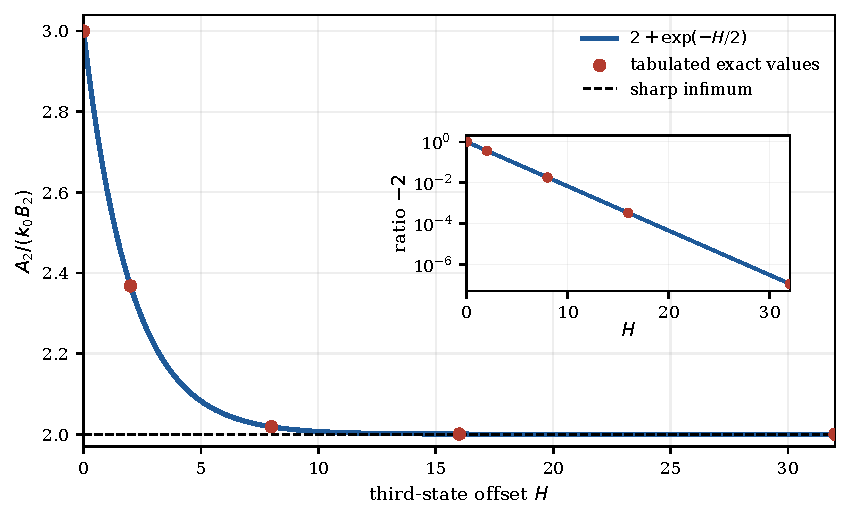
\includegraphics[width=0.78\linewidth]{sharpness.pdf}
 \caption{Exact sharpness family in Eq.~\eqref{eq:sharpfamily}. The solid curve and
 selected markers are generated from the analytic formula, not from a fit. The inset
 shows the positive margin above $2$ on a logarithmic scale. The dashed line is the
 uniform infimum and is reached only at the excluded $H=\infty$ limit.}
 \label{fig:sharpness}
\end{figure}

\section{Checks, interpretation, and limitations}
\label{sec:checks}

The proof above is exact. Numerical calculations were used only to detect convention
errors and to verify that the full nonlinear periodic solution approaches the modal
formula. One implementation evolves all three probabilities through a full-period
propagator. A second eliminates normalization and solves the remaining periodic equations
by Fourier collocation. Table~\ref{tab:checks} gives two fixed examples. Both use
$k_0=1$. The last column reports the larger of the absolute differences in $\Aobs$ and
$k_0\Bobs$ between the two representations at $\eps=0.05$; it is not an error bound for
the analytic theorem.

\begin{table}[ht]
\centering
\caption{Convention and perturbative checks. The linear-response (LR) ratio is computed
from Eqs.~\eqref{eq:B2}--\eqref{eq:A2}; the nonlinear ratio uses the full periodic state
at $\eps=0.025$.}
\label{tab:checks}
\small
\begin{tabular}{@{}lcccc@{}}
\toprule
case & $\Omega/k_0$ & LR $A_2/(k_0B_2)$ & nonlinear $\Aobs/(k_0\Bobs)$ & max. difference \\
\midrule
generic two-harmonic & $1.3$ & $3.3034360094$ & $3.3024363997$ & $1.47\times10^{-15}$ \\
offset family, $H=7$ & $0.8$ & $2.0301973834$ & $2.0302467618$ & $1.22\times10^{-17}$ \\
\bottomrule
\end{tabular}
\end{table}

The generic case uses offsets $(-0.8,0.3,1.1)$ and two sine/cosine harmonics; the second
uses offsets $(0,0,7)$ and an antisymmetric single-harmonic drive. In both cases all
probabilities remain positive, normalization and periodic closure are at roundoff, and
the scaled nonlinear observables converge to the separately evaluated coefficients as
$\eps$ decreases. The supplied scripts and captured outputs specify all coefficients,
tolerances, and collocation sizes.

Physically, Eq.~\eqref{eq:strictidentity} shows why merely adding the smallest cycle does
not produce excessive lag under fully symmetric kinetics in linear response. The
conductance weight $r_ir_j/Z$ of every edge dominates twice its contribution to the
equilibrium variance, with a strictly positive contribution from the third state. Each
relaxation channel is therefore faster than the symmetric two-state scale, and the phase
inherits the stronger bound through a positive modal average.

This conclusion has several precise limits. It is a leading-order result as
$\eps\to0$ for fixed finite input. It does not provide a uniform amplitude radius and
does not prove either the stronger or weaker inequality at arbitrary finite amplitude.
It also does not cover missing edges, asymmetric rate splitting, heterogeneous edge
prefactors, transient rather than periodic states, singular offsets, more than three
states, or a drive with unbounded harmonic content. Thus the original all-amplitude
complete-three-state question remains unresolved. Any violation there would have to be
a genuinely nonlinear-amplitude effect, not a failure already present in this symmetric
linear-response mechanism.

\section{Conclusion}

For the complete symmetric three-state Markov model, the leading weak-driving phase is
controlled by a positive average of two reversible relaxation rates. A strict
three-point Dirichlet identity places each rate above $2k_0$, proving the factor-two
phase-lag bound for arbitrary finite offsets and arbitrary non-gauge finite Fourier
driving. The constant is sharp only through an effective-two-state infinite-offset
limit. The result settles a coherent perturbative subdomain but leaves the source's
finite-amplitude multistate conjecture open.

\section*{Code and data availability}

No external data set is used. The reproducibility package contains the exact figure
script and tabulated values, a full-period three-coordinate propagator, an independent
two-coordinate Fourier-collocation solver, and a modal-response checker. The archived
environment is Python 3.12.14 with NumPy 2.3.5, SciPy 1.18.1, and Matplotlib 3.11.2.
The accompanying README gives regeneration commands and distinguishes numerical checks
from the analytic proof.

\section*{Acknowledgements and disclosure of AI assistance}

OpenAI Codex using model \texttt{gpt-5.6-sol} assisted with problem scoping, analytic
derivations, code generation and execution, numerical verification, literature
discovery, and preparation of this draft. A separately initialized session of the same
model reconstructed and stress-tested the central calculation. The AI system is not an
author. Before any submission, the named author must critically review the complete
manuscript, independently confirm the claims and references, and update this disclosure
as required by the target journal.

\bibliographystyle{unsrtnat}
\bibliography{references}

\end{document}
